\subsection{NEON Single String Testbed}
The National Ecological Observatory Network (NEON) is an designed to facilitate an advanced understanding of how ecosystems and organisms respond to variations in climate and changes 
in land use. To validate various aspects of the NEON architecture with working prototypes, 
NEON Single-String Diagnostic Testbed (SSTB) activity was initiated. We now describe SSTB and explain how we have used RBNB DataTurbine in this deployment. The goal of the SSTB activity was to develop an end-to-end prototype that streams data from the NEON Wireless Platform (NWP) deployed at a field station 
% UCR/James Reserve
 using a streaming data middleware to a database system deployed at a data center. Figure~\ref{fig: ssarch} shows where individual components are
located -- in field station and data center. The field station and the data center are about 
100 miles apart from each other.
% San Diego Supercomputer Center. 

\begin{figure*}
% \begin{center}
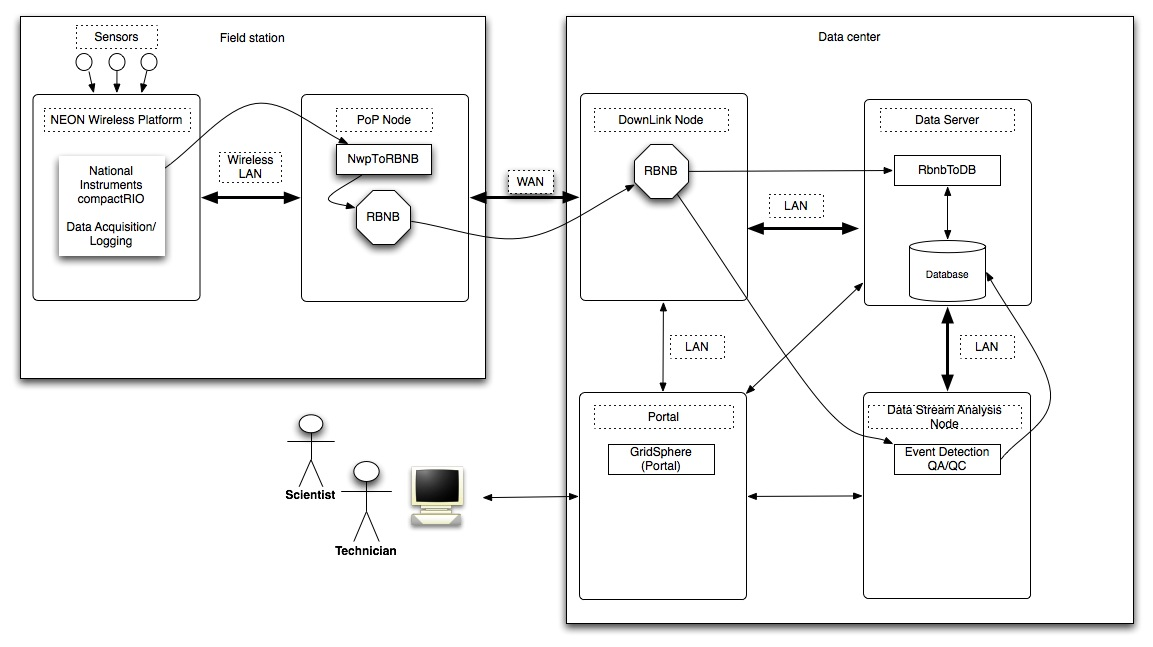
\includegraphics[scale=0.40]{figs/ssarch}
% \end{center}
\caption{\label{fig: ssarch}
NEON Single String Testbed}
\end{figure*}

The Compact RIO is an embedded data acquisition platform manufactured by National Instruments.
In the prototype phase, a Compact RIO datalogger with wireless (802.11b) extensions has been selected as the NEON Wireless Platform (NWP) for  data acquisition system for prototyping. As a part of SST activity, our collaborators deployed a NWP along with Vaisala Weather Transmitter WXT510 and Vaisala Digital Barometric Pressure Sensor (PTB210) at the the field station. Our collaborators 
developed the device driver in LabVIEW for collecting data from the aforementioned sensors connected to the NWP. We deployed PoP node  at the field station. The PoP node hosts an RBNB server and a RBNB source program called NwpToRbnb (ref. Figure~\ref{fig: ssarch}). NwpToRbnb is a Java program that acts as a gateway and facilitates dataflow from the NWP to the RBNB server on the PoP node. It accomplishes this by querying the NWP for data and metadata, processing these items, and then forwarding this data and metadata to the RBNB server deployed on the PoP node. This program initiates the connection with the NWP using sockets and uses standard TCP/IP networking protocols to communicate with the NWP over the wireless channel. Once the session is established, then data is transmitted in an event-driven manner from the NWP to the PoP. 

\emph{Downlink Node:} This 
 % -- San Diego Supercomputer Center. Downlink node
hosts a RBNB server, which runs as the parent node for the RBNB server running on the PoP node. RBNB server running on the downlink node provides access to real-time data streams for various clients. For example, as shown in Figure~\ref{fig: ssarch}, we can fork data streams from the RBNB server running at the downlink node to applications running on the data stream analysis node and data server node.
	
\emph{Data Server node:} This hosts a PostgreSQL database. RbnbToDb is a DataTurbine sink (ref. Figure~\ref{fig: ssarch})that runs in subscription mode. RbnbToDb program connects to RBNB server on the downlink node, extracts the data and then inserts it into the database. RbnbToDb utilizes the JDBC abstraction layer, so the use of Postgres is subject to later revision as requirements change.

\emph{Data stream analysis node:}
 We are currently working on providing this functionality. This node is designed to host software infrastructure that can perform analysis on real-time data streams. An example of such software is Kepler~\cite{kepler} and examples of analysis routines are event detection and QA/QC.
 
\emph{Web Portal node:}
Web portal node hosts the portal software infrastructure. We have deployed a GridSphere-based portal infrastructure, with portlets to support different functions, e.g. for login, and data access/display.

At present the RBNB servers running on the PoP node and the downlink node have been
buffering approximately  one weeks' worth of data. So far in this deployment we have found RBNB DataTurbine to be very robust.
